\section{实证证据}

\begin{frame}{样本与识别策略}
  好，现在来看数据。我们的样本是 2009--2023 年的 A 股上市公司。

  \vspace{0.4em}
  识别策略是交叠双重差分，核心设定是：
  \[
    Y_{it}=\alpha_i+\gamma_t+\beta D_{it}
    +\Gamma X_i \times f(t)+\varepsilon_{it}.
  \]

  \begin{itemize}
    \item $D_{it}$ 是企业 $i$ 在 $t$ 年是否已通过贯标认证；
    \item $\alpha_i$ 和 $\gamma_t$ 分别控制企业固定效应和年份固定效应；
    \item 识别来自于\emph{同一家企业贯标前后的投资结构变化}，同时由尚未贯标的企业提供对照。
  \end{itemize}

  \vspace{0.4em}
  $X_i\times f(t)$ 是事前特征与年份三次多项式的交乘——这么做的目的是在控制事前差异的同时，避免把政策后的变量当成坏控制。
\end{frame}

\begin{frame}{贯标企业的进入时间分布}
  \begin{figure}
    \centering
    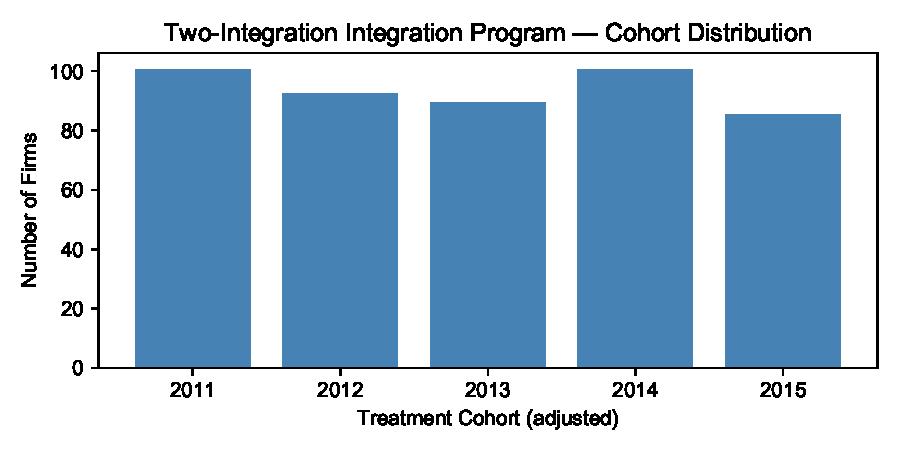
\includegraphics[width=0.65\linewidth,height=0.68\textheight,keepaspectratio]{figures/paper/Cohort_Distribution.pdf}
    \caption{各批次贯标企业的数量分布}
  \end{figure}
\end{frame}

\begin{frame}{为什么不能假设"无预期"？}
  前面提到过，两化融合不是突发冲击。如果忽略预期效应，事前系数就会被污染。

  \vspace{0.4em}
  我们的处理方式是：
  \begin{itemize}
    \item 把有效处理起点前移到认证通过日之前若干期；
    \item 用事前趋势诊断和有限预期窗口，把预期效应和实际处理效应分开。
  \end{itemize}

  \vspace{0.4em}
  具体来说，我们估计：
  \[
    Y_{it}=\alpha_i+\gamma_t
    +\sum_{l=-K_1}^{-2}\mu_lD_{it}^{l}
    +\sum_{l=0}^{K_2}\mu_lD_{it}^{l}
    +\Gamma X_i\times f(t)+\varepsilon_{it}.
  \]
\end{frame}

\begin{frame}{事件研究：预期被适当处理后}
  \begin{figure}
    \centering
    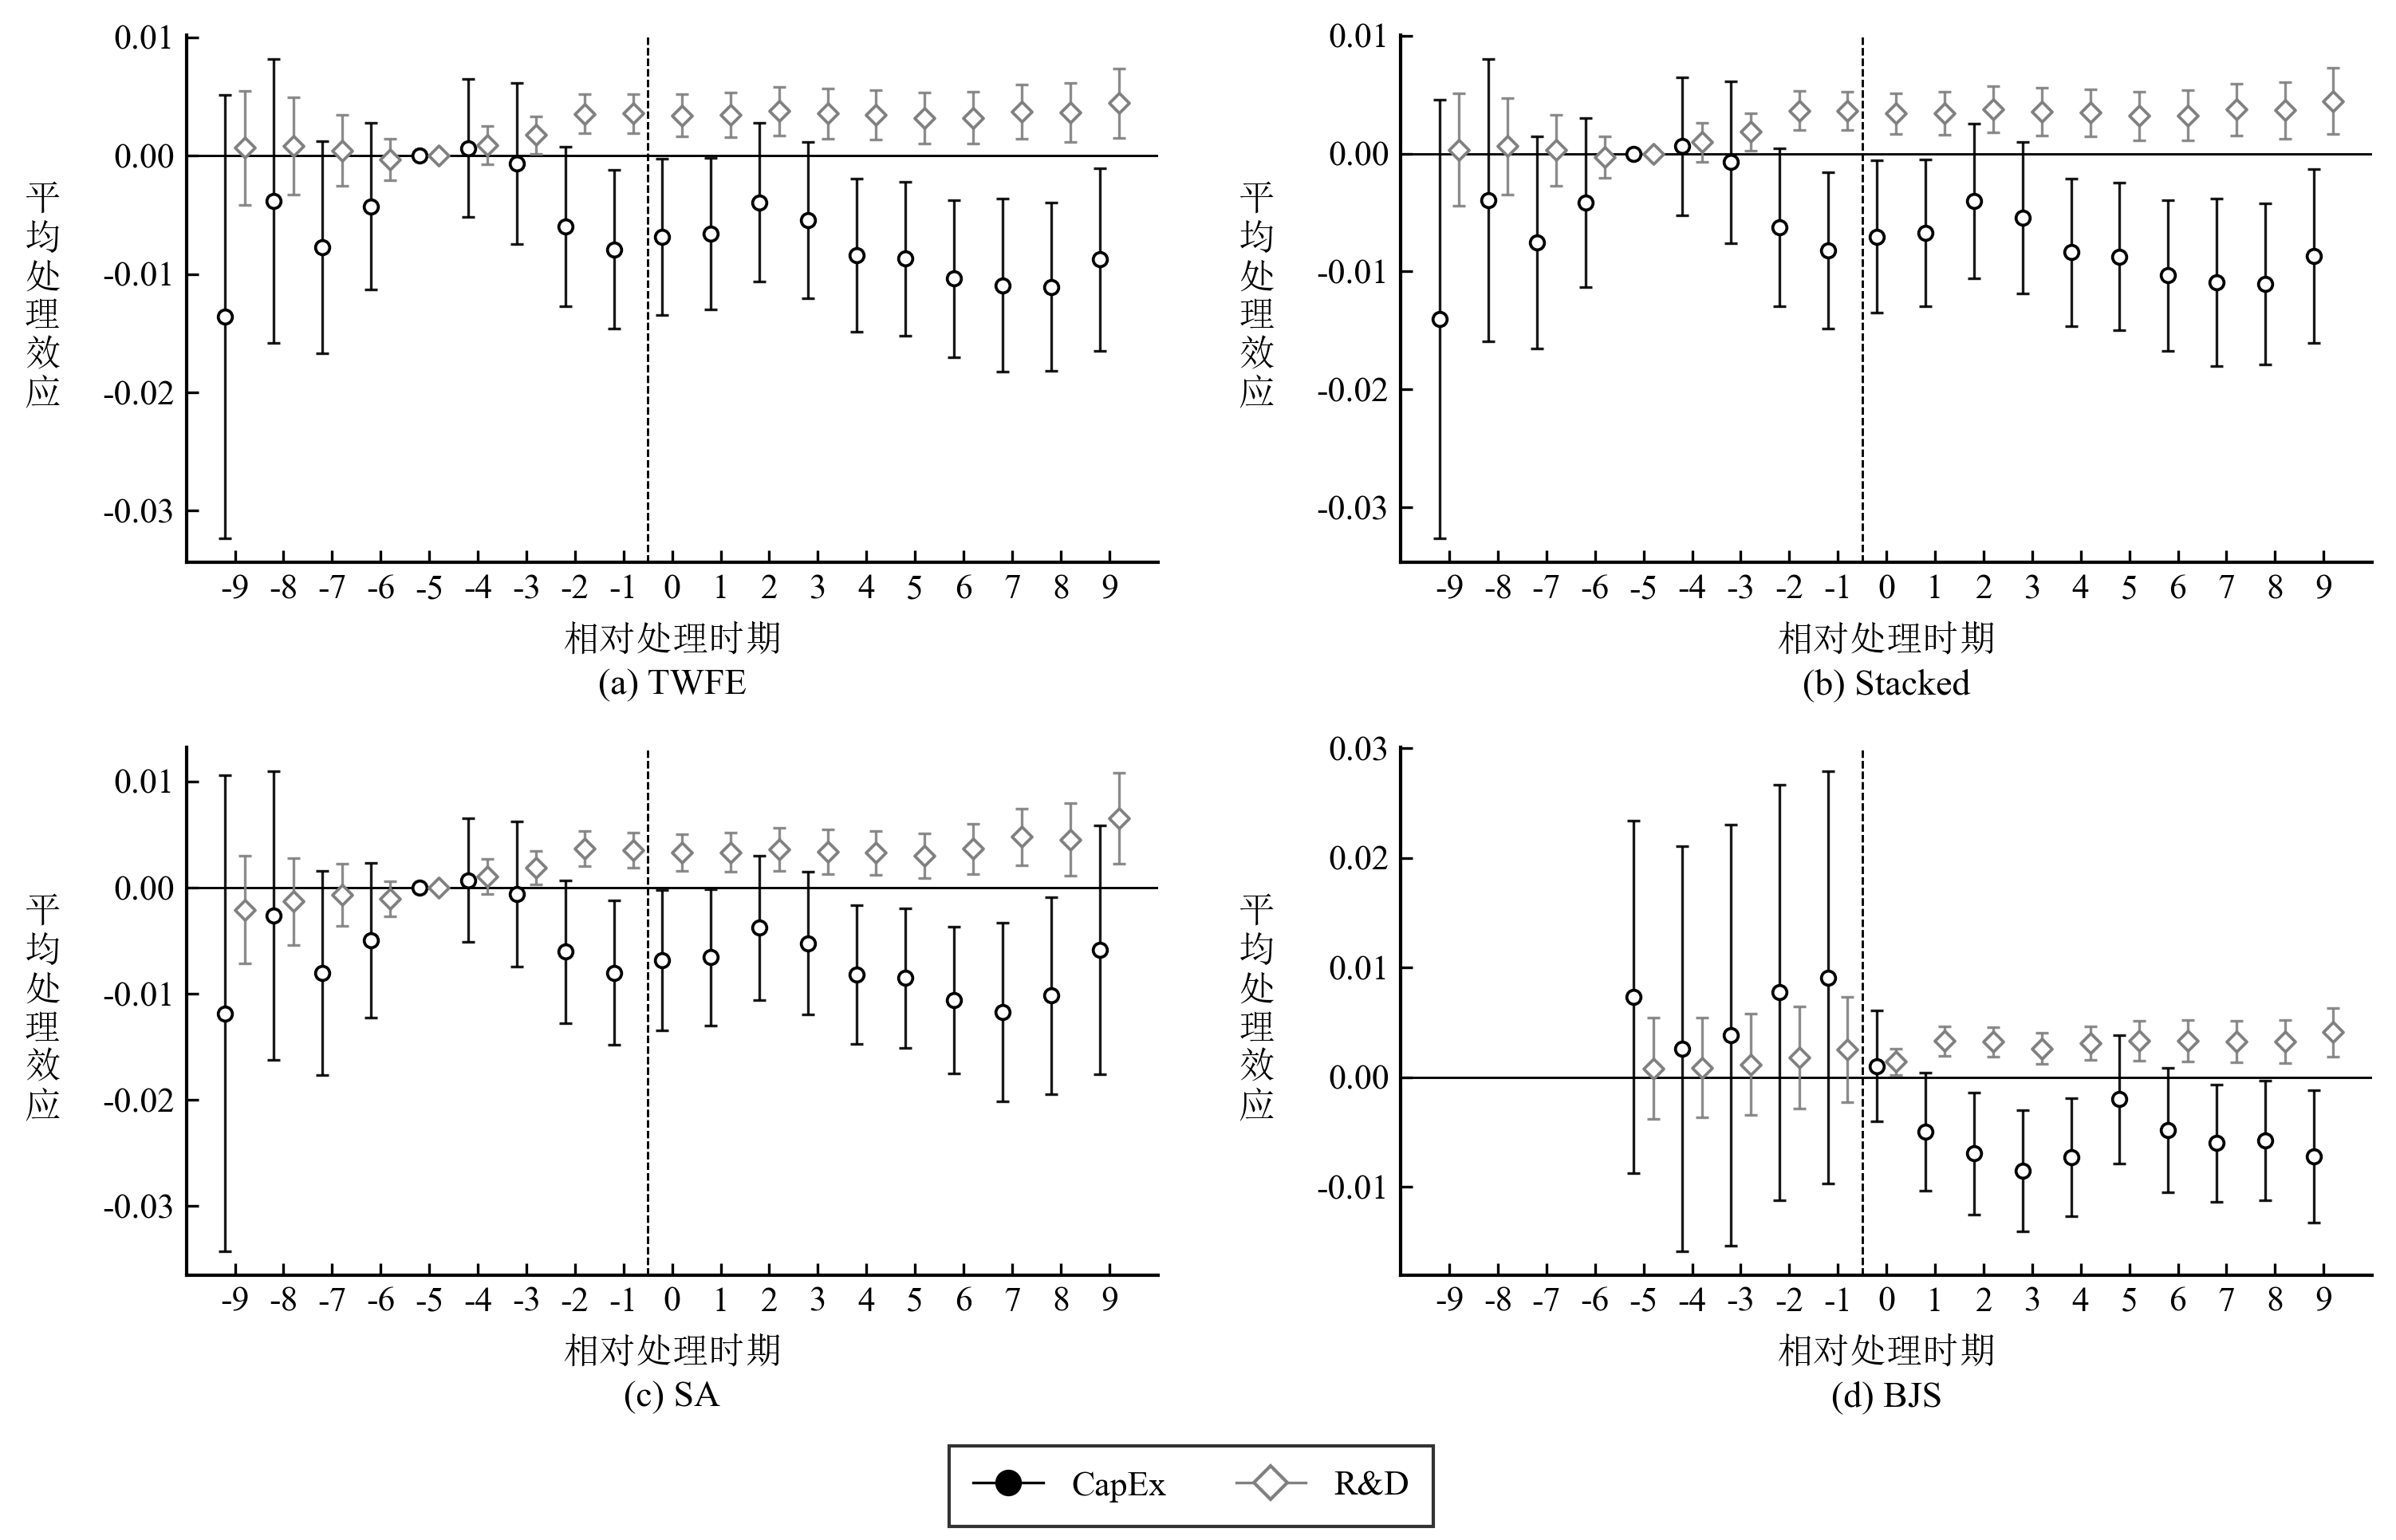
\includegraphics[width=0.86\linewidth,height=0.68\textheight,keepaspectratio]{figures/paper/anticipation-event-study.png}
    \caption{控制有限预期窗口后的事件研究：左为 CapEX，右为 R\&D}
  \end{figure}
\end{frame}

\begin{frame}{基准结果：一降一升}
  {\scriptsize
\begin{center}
\begin{tabular}{lcccc}
  \toprule
  变量 & (1) CapEX & (2) CapEX & (3) R\&D & (4) R\&D \\
  \midrule
  两化融合 & $-0.006^{**}$ & $-0.005^{**}$ & $0.003^{***}$ & $0.003^{***}$ \\
             & (0.002) & (0.002) & (0.001) & (0.001) \\
  控制变量 & 否 & 是 & 否 & 是 \\
  个体固定效应 & 是 & 是 & 是 & 是 \\
  时间固定效应 & 是 & 是 & 是 & 是 \\
  样本量 & 44,762 & 44,759 & 44,789 & 44,786 \\
  调整 $R^2$ & 0.493 & 0.496 & 0.819 & 0.820 \\
  \bottomrule
\end{tabular}
\end{center}
}


  \vspace{0.4em}
  \begin{findingbox}{经济含义}
    贯标后，企业实物投资水平相对于均值下降了约 \textbf{9.8\%}，而研发支出相对于均值上升了约 \textbf{14.3\%}。
  \end{findingbox}

  \vspace{0.3em}
  方向完全符合模型的第一个预测——实物投资降，研发投入升。
\end{frame}

\begin{frame}{这个"剪刀差"长什么样？}
  \begin{figure}
    \centering
    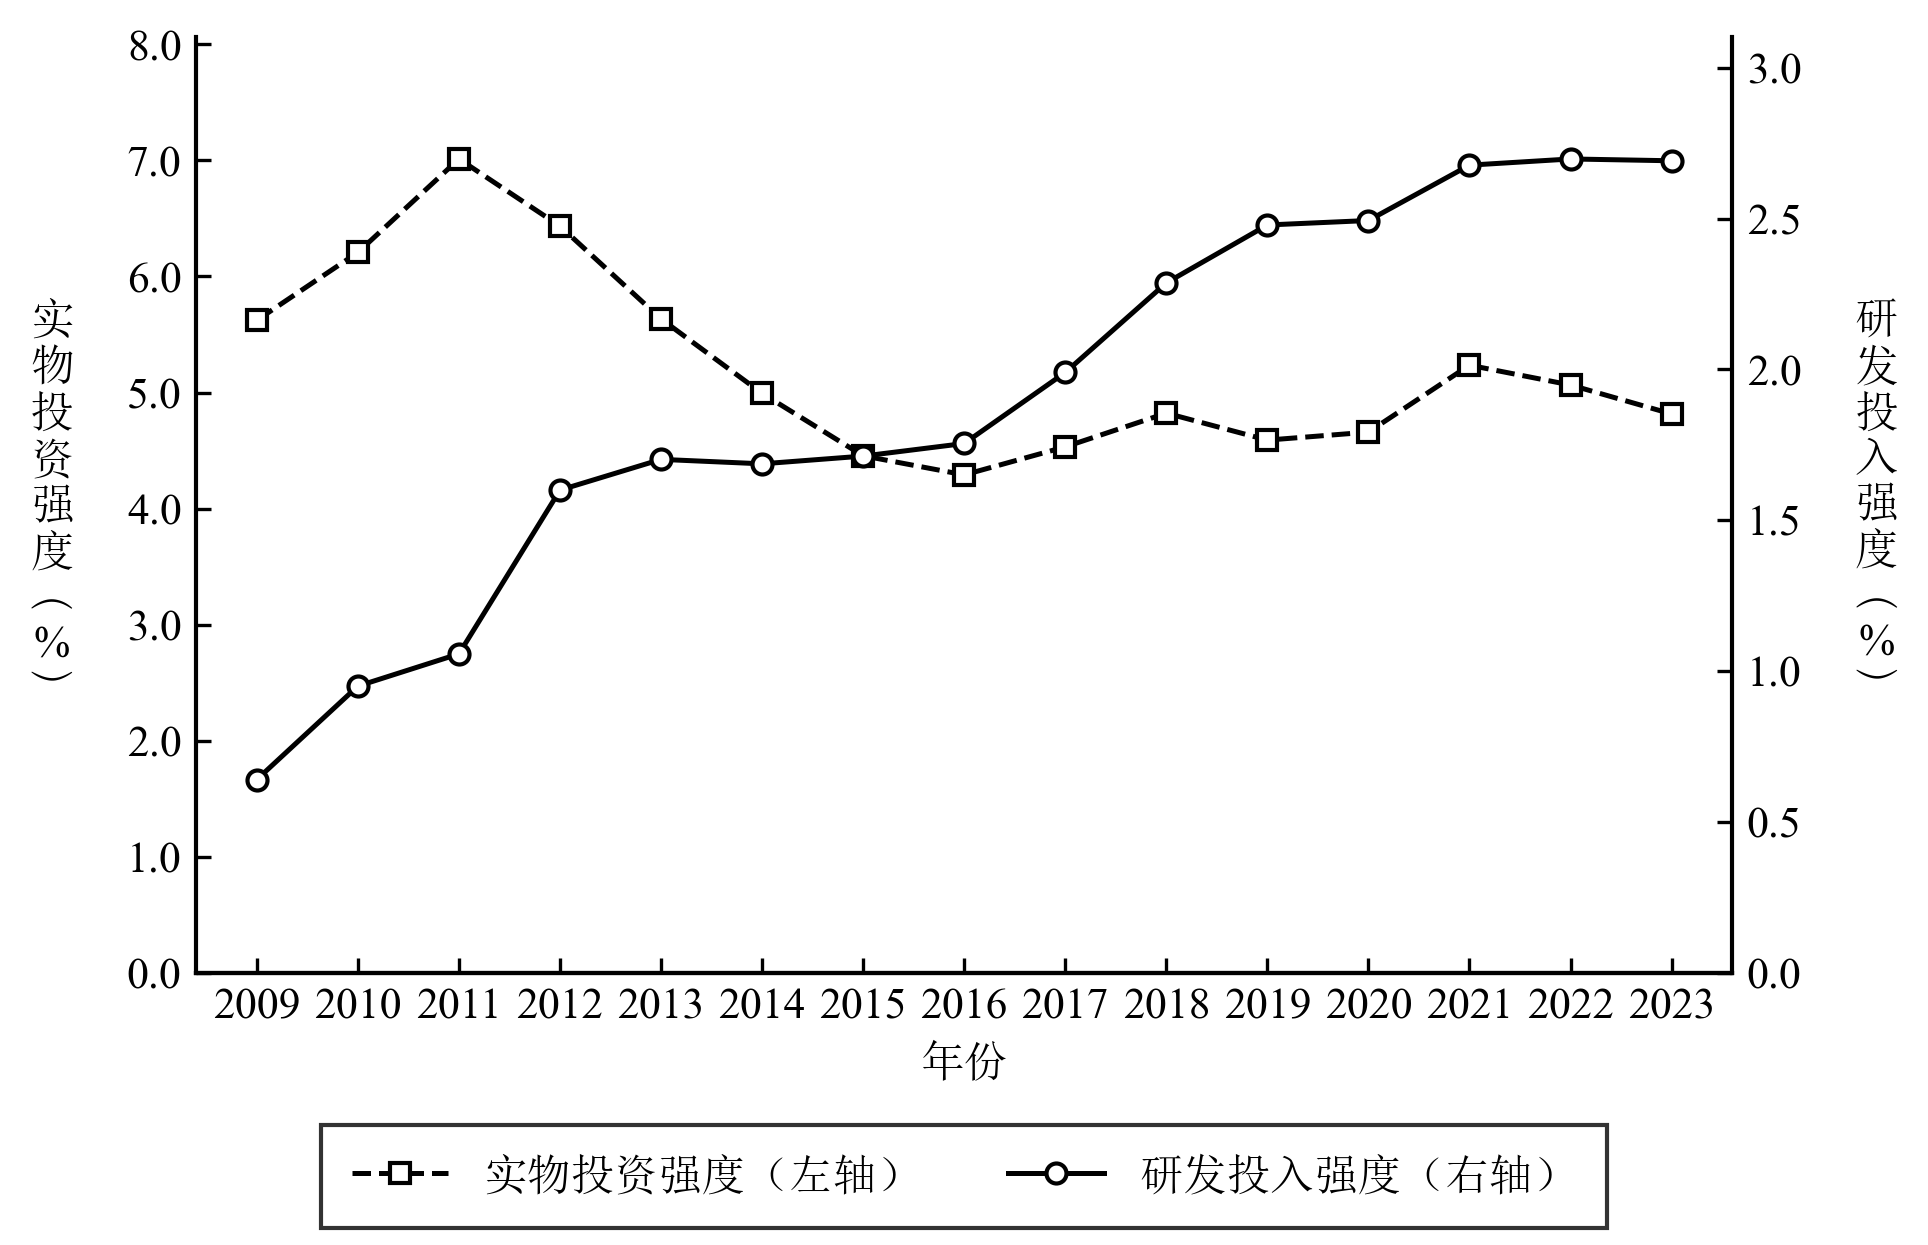
\includegraphics[width=0.78\linewidth,height=0.62\textheight,keepaspectratio]{figures/paper/micro-investment-structure.png}
    \caption{上市企业层面，实物投资与研发投入的分化趋势}
  \end{figure}
\end{frame}

\begin{frame}{稳健性：换估计量、换样本、换设定}
  基准结果稳不稳？我们做了以下检验：

  \begin{itemize}
    \item 使用 Sun--Abraham、Callaway--Sant'Anna、Borusyak--Jaravel--Spiess 等异质性稳健估计量，结论不变；
    \item PSM-DID、合成控制 DID、堆叠 DID 的结果一致；
    \item 控制投入产出网络溢出后，结论仍在。
  \end{itemize}

  \vspace{0.5em}
  我们还专门排除了几个竞争性解释：
  \begin{itemize}
    \item 控制供给侧去产能、金融去杠杆、房地产价格波动等宏观冲击后，CapEX 降、R\&D 升的结论没有变化。
  \end{itemize}
\end{frame}

\begin{frame}{稳健性：多估计量对比与安慰剂检验}
  \begin{figure}
    \centering
    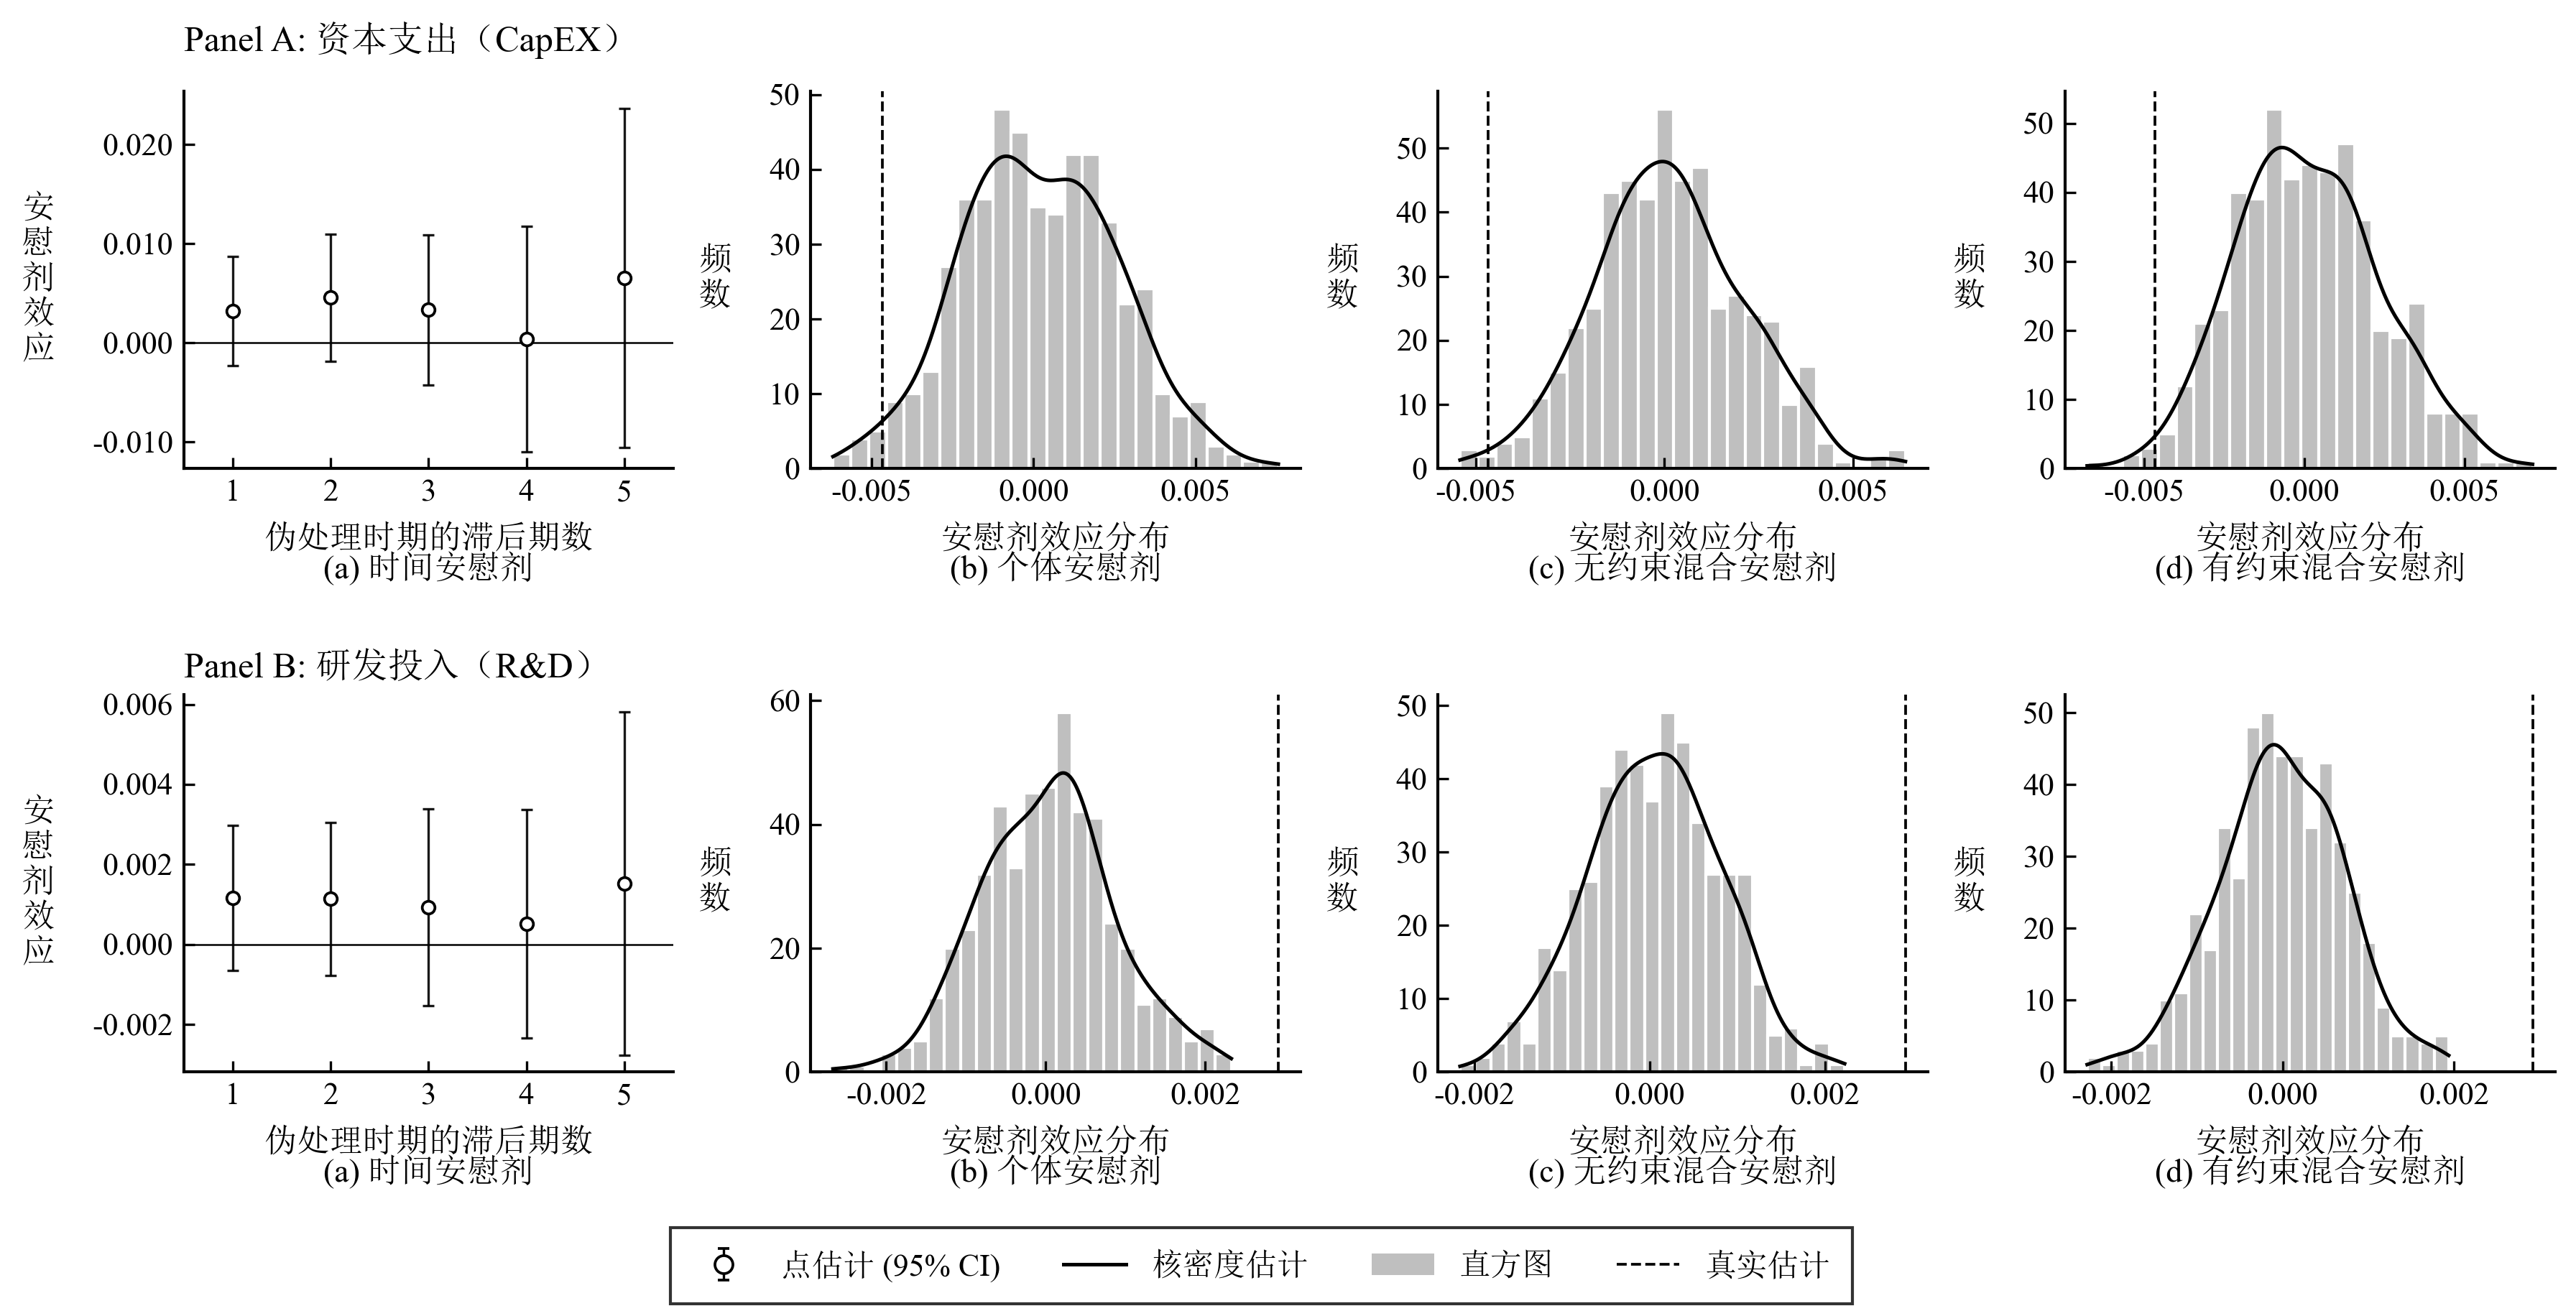
\includegraphics[width=0.8\linewidth,height=0.68\textheight,keepaspectratio]{figures/paper/placebo-tests.png}
    \caption{安慰剂检验与多种异质性稳健估计量的对比}
  \end{figure}
\end{frame}

\begin{frame}{机制一：怎么度量"抵押囤积"？}
  模型的第二个预测是：CapEX 收缩应该集中在那些事前囤积了大量超额资本的企业。

  \vspace{0.4em}
  怎么衡量"囤积"？我们构造了一个\emph{事前囤积楔子 PH}：
  \[
    \ln K_{it}
    =
    \beta_0+\beta_1\ln Y_{it}+\beta_2\ln L_{it}
    +\beta_3\text{SalesGrowth}_{it}
    +\alpha_j+\gamma_t+\varepsilon_{it}.
  \]

  \begin{itemize}
    \item 残差 $\varepsilon_{it}$ 就是控制产出、劳动和成长机会后仍然"多余"出来的那部分资本；
    \item 把企业层面的事前残差均值标准化，就得到了 PH——数值越大，囤积越严重。
  \end{itemize}
\end{frame}

\begin{frame}{机制一：囤积越多的企业，收缩越剧烈}
  {\scriptsize
\begin{center}
\begin{tabular}{lcccc}
  \toprule
  变量 & 抵押率 & CapEx & 抵押率 & 在建工程/总资产 \\
  \midrule
  PH & $0.0426^{***}$ &  &  &  \\
     & (0.0093) &  &  &  \\
  两化融合 &  & $-0.0051^{**}$ & 0.0289 & $-0.0018$ \\
           &  & (0.0023) & (0.0198) & (0.0025) \\
  两化融合 $\times$ PH &  & $-0.0172^{***}$ & $-0.0503^{**}$ & $-0.0135^{***}$ \\
                       &  & (0.0026) & (0.0217) & (0.0035) \\
  控制变量与双向 FE & 是 & 是 & 是 & 是 \\
  调整 $R^2$ & 0.408 & 0.417 & 0.537 & 0.388 \\
  \bottomrule
\end{tabular}
\end{center}
}


  \vspace{0.4em}
  两点发现：
  \begin{itemize}
    \item PH 与事前抵押率显著正相关——说明 PH 确实在捕捉抵押融资依赖，不是随便定义的指标；
    \item PH 每高出一个标准差，贯标对资本支出的收缩效应额外增加约 \textbf{1.7 个百分点}——这大约是基准主效应的\emph{三倍}。
  \end{itemize}
\end{frame}

\begin{frame}{出清发生在哪里？边际投资，不是存量甩卖}
  \begin{itemize}
    \item 把有形资本按抵押属性拆开后，交互项的负效应主要集中在\emph{在建工程}——抵押属性最弱的科目；
    \item 固定资产、投资性房地产等高粘性存量资产，反应并不显著。
  \end{itemize}

  \vspace{0.5em}
  \begin{findingbox}{这个细节很重要}
    囤积型企业并不是在变卖厂房和设备，而是\emph{停止追加新的资本形成}。出清通过控制边际投资流量实现，而不是通过甩卖既有存量——这和 Shleifer--Vishny（1992）讲的资产流动性折价逻辑是一致的。
  \end{findingbox}
\end{frame}

\begin{frame}{机制二：信息替代抵押——企业端证据}
  现在看模型的第三个预测：信息替代抵押的逻辑在数据上是否成立。

  \vspace{0.4em}
  我们构造了一个\emph{剩余抵押空间}指标：
  \[
    \text{Slack}_{it}
    =
    \overline{\text{MR}}_{j,p90}^{2011}
    -
    \text{MR}_{it}.
  \]

  \begin{itemize}
    \item $\text{MR}_{it}$ 是企业实际的抵押率，$\overline{\text{MR}}_{j,p90}^{2011}$ 是行业在 2011 年的第 90 百分位；
    \item 差值越大，说明企业离行业抵押天花板越远，传统抵押空间越充裕；
    \item 差值越小甚至为负——说明企业已经快要触及传统抵押上限了。
  \end{itemize}
\end{frame}

\begin{frame}{机制二：越接近抵押上限，信贷扩张越强}
  {\scriptsize
\begin{center}
\begin{tabular}{lcccc}
  \toprule
  变量 & 总贷款 & 抵押贷款 & 短期贷款 & 长期贷款 \\
  \midrule
  两化融合 & $0.363^{***}$ & $0.370^{***}$ & $0.319^{***}$ & $0.250^{**}$ \\
           & (0.069) & (0.113) & (0.073) & (0.112) \\
  两化融合 $\times$ 剩余抵押空间 & $-0.204^{**}$ & $-0.265^{*}$ & $-0.205^{**}$ & $-0.163$ \\
                                      & (0.099) & (0.152) & (0.101) & (0.172) \\
  \bottomrule
\end{tabular}
\end{center}
}


  \vspace{0.3em}
  \begin{itemize}
    \item 两化融合与剩余抵押空间的交互项\emph{显著为负}；
    \item 也就是说，越逼近抵押天花板、传统抵押空间越紧张的企业，从贯标中获得的信贷扩张反而越大。
    \item 这恰好是"信息替代抵押"应该看到的模式——而不是泛泛地降低信息不对称。
  \end{itemize}
\end{frame}

\begin{frame}{机制二：银行端证据——竞争更激烈的市场更依赖硬信息}
  {\scriptsize
\begin{center}
\begin{tabular}{lcccc}
  \toprule
  变量 & 总贷款 & 抵押贷款 & 短期贷款 & 长期贷款 \\
  \midrule
  两化融合 & $0.501^{***}$ & $0.662^{***}$ & $0.403^{***}$ & $0.384^{**}$ \\
           & (0.120) & (0.179) & (0.119) & (0.162) \\
  两化融合 $\times$ 银行竞争度（CR3） & $-0.386^{**}$ & $-0.723^{***}$ & $-0.340^{**}$ & $-0.312$ \\
                                      & (0.155) & (0.243) & (0.166) & (0.210) \\
  \bottomrule
\end{tabular}
\end{center}
}


  \vspace{0.3em}
  \begin{itemize}
    \item 银行集中度高的市场，更容易通过长期银企关系生产\emph{软信息}；
    \item 竞争激烈的市场，银行更依赖\emph{硬信息}和抵押品。
    \item 结果很清楚：贯标的信贷促进作用，在银行竞争越激烈、关系型软信息越稀缺的地区\emph{越强}。
  \end{itemize}

  \vspace{0.3em}
  企业端和银行端的证据，从两边共同支撑了"信息替代抵押"的机制。
\end{frame}

\begin{frame}{效率含义：资本错配改善了吗？}
  最后看效率。如果投资结构调整只是被动缩表，我们不应该看到配置效率的改善。

  \vspace{0.4em}
  用标准的 MRPK 离散度来衡量资本错配：
  \[
    MRPK_{it}
    =
    \frac{\partial \text{Revenue}_{it}}{\partial K_{it}}
    =
    \alpha_K^j\cdot\frac{\text{Revenue}_{it}}{K_{it}}.
  \]

  {\scriptsize
\begin{center}
\begin{tabular}{lccc}
  \toprule
  变量 & (1) MRPK & (2) CapEx & (3) CapEx \\
  \midrule
  两化融合 & $0.099^{**}$ & $-0.007^{**}$ & 0.002 \\
           & (0.050) & (0.003) & (0.003) \\
  两化融合 $\times$ High MRPK & $-0.382^{***}$ &  &  \\
                              & (0.064) &  &  \\
  两化融合 $\times Q_{t-1}$ &  & $0.006^{***}$ &  \\
                              &  & (0.002) &  \\
  两化融合 $\times$ 资本年龄$_{t-1}$ &  &  & $-0.004^{**}$ \\
                                      &  &  & (0.002) \\
  双向 FE + 高维交互 FE & 是 & 是 & 是 \\
  \bottomrule
\end{tabular}
\end{center}
}

\end{frame}

\begin{frame}{效率改善的三条证据}
  \begin{itemize}
    \item 事前 MRPK 较高的企业在政策后出现更强的边际回报回落，行业内的 MRPK 离散度\emph{显著下降}——资本在向回报更高的地方流动；
    \item 尽管企业总体资本支出规模在收缩，投资对滞后一期 Tobin's $Q$ 的敏感性反而\emph{上升}——说明投资筛选质量在变好；
    \item 资本年龄越高，贯标对实物资本支出的抑制效应就越强——跟模型预测的"老资本更容易掉进囤积区域"完全吻合。
  \end{itemize}

  \vspace{0.5em}
  三条证据合在一起，指向同一个结论：\emph{这不是被动紧缩，而是资本配置效率在改善}。
\end{frame}

\begin{frame}{研发不只是费用：从短期支出到长期资产}
  {\scriptsize
\begin{center}
\begin{tabular}{lccccc}
  \toprule
  变量 & 创新补助 & 员工数 & 研发人员占比 & 费用化率 & 资本化率 \\
  \midrule
  两化融合 & $0.457^{***}$ & $0.090^{**}$ & $6.954^{***}$ & $-3.145^{*}$ & $5.923^{*}$ \\
           & (0.086) & (0.036) & (2.425) & (1.853) & (3.085) \\
  \bottomrule
\end{tabular}
\end{center}
}


  \vspace{0.3em}
  最后一个机制证据：贯标之后，企业的研发活动发生了什么变化？

  \begin{itemize}
    \item 创新补助显著增加，研发人员占比上升——研发的\emph{"量"}在扩大；
    \item 更值得关注的是结构变化：研发费用化比率下降、资本化比率上升——说明研发在从短期分散投入，转向更制度化、可持续的长期资产构建。
  \end{itemize}
\end{frame}
